\documentclass[12pt,a4paper]{report} % Use report class for thesis
\usepackage[utf8]{inputenc}           
\usepackage{setspace}                 
\usepackage{graphicx}                 
\usepackage{caption}                  
\usepackage{geometry}                 
\usepackage{fancyhdr}                 
\usepackage{natbib}                   
\usepackage{hyperref}  
 \usepackage{etoolbox}
 \makeatletter
 \pretocmd{\contentsline}{\begingroup\hypersetup{hidelinks}}{}{}
 \apptocmd{\contentsline}{\endgroup}{}{}
 \pretocmd{\addcontentsline}{\begingroup\hypersetup{hidelinks}}{}{}
 \apptocmd{\addcontentsline}{\endgroup}{}{}
 \makeatother             
\usepackage{booktabs}                 
\usepackage{xcolor}
\usepackage{graphicx}
\usepackage{setspace}
\usepackage{geometry}
\usepackage{attachfile2}  % to attach files
\usepackage{tcolorbox}      % colored boxes
\usepackage{fontawesome5}   % optional icons
\usepackage{appendix}       % for appendix support




\geometry{top=3cm, bottom=3cm, left=2.5cm, right=2.5cm} 

% Header and footer
\pagestyle{fancy}
\fancyhf{}
\fancyhead[L]{\leftmark}   
\fancyhead[R]{\thepage}    
\renewcommand{\headrulewidth}{0.5pt}



\begin{document}
	
	% Double spacing
	\onehalfspacing
	
	\begin{titlepage}
		\centering
		
		% University Logo
\begin{figure}
	\centering
	
\includegraphics[width=0.4\linewidth]{screenshot021}
	\end{figure}
		% Replace 'university_logo.png' with the actual file name of your logo
		
		% Title
		{\LARGE \bfseries Forecasting Sri Lanka's Commodity Net 
			Export Price Index Using ARIMA Models \par}\vspace{2cm}
		
		% Author
		{\large By \par}
		{\Large \bfseries Datafora  \par}
		{\large Group 01 \par}\vspace{1.5cm}
		
		% Submission Text
		{\large Presented to: \par}
			{\Large \bfseries Dr. Neluka Devpura  \par}\vspace{1.0cm}
			
		{\Large \bfseries STA 3512 / ASP 4582 Research
			Methodology \par}
		
		% Department Info
		{\large Department of Statistics \par}
		{\large Faculty of Applied Sciences \par}
		{\large of the \par}
		{\Large \bfseries University of Sri Jayewardenepura \par}
		{\large Nugegoda \par}
		{\large Sri Lanka \par}
		
		\vfill
		
	\end{titlepage}
	
	% Double spacing
	\doublespacing
	
	% Customize captions: smaller font and italic
	\captionsetup{
		font={footnotesize,it},  % smaller font than 'small'
		labelfont=it,
		labelsep=colon
	}
	
	
	\clearpage
	
	% ===== Group Details Table (No Page Number) =====
	\thispagestyle{empty} % Removes page number from this page
	\begin{center}
		\section*{Group Member Details} % Unnumbered section, not added to TOC
		
		\begin{tabular}{|c|l|l|}
			\hline
			\textbf{Index No} & \textbf{Name} & \textbf{Email} \\ \hline
			AS2022399
			 & S.G.V.S.Samaranayaka & sgvinudiss@gmail.com \\ \hline
			AS2022404
			 & I.V.N.N.Wijesekara & nawanjanawijesekara2001@gmail.com \\ \hline
			AS2022409 
			 & G.R.Jayasinghe & ranindeejayasinghe@gmail.com \\ \hline
			AS2022423  & S.S.Balasooriya  & sajani2023balasooriya@gmail.com \\ \hline
			AS2022556
			 & M.N.D.Gunarathna & nethminidivyangana1218@gmail.com \\ \hline
			AS2022577 
			 & N.G.S.Minimuthu & sheharaminimuthu@gmail.com \\ \hline
			AS2022642 & Y.M.A.P.Rajapaksha & amali2022ugc@gmail.com \\ \hline
		\end{tabular}
	\end{center}
	
	\clearpage
	
	
	%============================
	% Switch to Roman page numbers for front matter
	%============================
	\pagenumbering{roman}  % i, ii, iii, ...
	\setcounter{page}{1}    % Start from i
	
	
	% Acknowledgements (after title page, before TOC)
	\chapter*{Acknowledgements}
	We would like to express our deepest gratitude to everyone who has supported and guided us throughout the completion of this research on forecasting Sri Lanka’s commodity net export price index using ARIMA model.
	
	First, we sincerely thank Dr. Neluka Devpura, our course instructor for STA 3512/ASP 4582 Research Methodology, for her invaluable guidance, support, and encouragement throughout this research. Her expertise, continuous support, suggestions and insightful feedback at every stage were invaluable in shaping the direction of our research and overcoming challenges we faced.
	
	We also extend our sincere appreciation to all other lecturers in statistic department who guided us throughout these years for providing a strong foundation that enabled us to effectively complete this research.We would like to extend our gratitude to department of statistics of faculty of applied sciences, University of Sri Jayewardenepura for providing us with the platform and academic resources to undertake this study.

	We acknowledge the International Monetary Fund (IMF) for making their database publicly available, which is used as the data source for the analysis.
	
	We would also like to acknowledge the researchers and authors whose prior studies in the area of time series analysis, ARIMA modeling and commodity net export price index forecasting provided the foundation and insights for our research.
	
	Finally, we express our deepest thanks to our group members for their commitment, collaboration, and team spirit. Their contributions, discussions, and dedication made this research possible and successful.
	
	
	% Add Acknowledgements to the table of contents
	\addcontentsline{toc}{chapter}{Acknowledgements}
	
	
	% Table of contents
	\tableofcontents
	\addcontentsline{toc}{chapter}{Contents}
	
	\listoffigures     % Generates List of Figures
	\addcontentsline{toc}{chapter}{List of Figures}
	
	\listoftables
	\addcontentsline{toc}{chapter}{List of Tables} 
	
	\chapter*{Abstract} % Abstract without chapter number
	\addcontentsline{toc}{chapter}{Abstract} % Add Abstract to TOC
	
	International trade plays a central role in the economy of Sri Lanka making the study of macroeconomic variables such as export, import and net export essential for economic forecasting, policy formulating and strategy planning. Hence this study focuses on forecasting Commodity Net Export Price Index (CNEPI) of Sri Lanka, weighting individual commodity prices with their ratio of net export to GDP. Monthly data from January 1980 to March 2025 which were obtained from International Monetary Fund (IMF) commodity terms of trade database are analyzed using several candidate Auto Regression Integrated Moving Average (ARIMA) models to find the statistically adequate model ARIMA (2,1,3). Applying (ARIMA) model to CNEPI which provides accurate forecast and valuable insights into relationship between trade and economic state of the country. This study aims to forecast Sri Lanka’s CNEPI for the period April 2025 to March 2026 using ARIMA model. Results revealed a gradual upward trend in CNEPI for the aimed forecasting time period indicating an improving in Sri Lanka’s trade conditions. The findings of this study show the importance of ARIMA models in economic forecasting for policymakers and businesses for efficient economic planning in Sri Lanka.
	
	
	
	%============================
	% Switch to Arabic page numbers for main chapters
	%============================
	\clearpage
	\pagenumbering{arabic}  % 1, 2, 3, ...
	\setcounter{page}{1}    % Start main chapters from 1
	

	\chapter{Introduction}
	
	International trade is one of the most important drivers of economic growth for any country in the modern world. No country can produce all the goods and services it needs by itself. Because of this, countries engage in trade with one another, exchanging what they produce in surplus for what they cannot produce efficiently at home. This trade mainly takes place in two directions, known as exports and imports. Exports are the goods and services that a country sells to foreign markets, while imports are the goods and services purchased from abroad. Together, they determine the strength of a nation’s economic ties with the rest of the world and play a major role in shaping national income, employment opportunities, and living standards.
	
	Exports are particularly important because they bring foreign exchange into the country. This foreign income is essential to pay for imports and to maintain stability in the balance of payments. A strong export sector also helps local producers to improve their production efficiency, adopt new technologies, and compete in global markets. For small economies like Sri Lanka, export growth is directly linked to economic development. Higher exports allow for industrial expansion, creation of new jobs, and improvement of living standards. Imports, on the other hand, can be both beneficial and challenging. They provide access to goods and services that are either not produced domestically or are too costly to produce locally. For instance, machinery, petroleum, raw materials, and advanced technology are commonly imported to support domestic industries. At the same time, too much dependency on imports can lead to trade deficits, foreign debt, and economic instability.
	
	The combined effect of exports and imports is measured by net exports, which is the difference between the two. When the value of exports exceeds the value of imports, the country records a trade surplus, which is generally favorable because it strengthens the economy and increases foreign reserves. On the other hand, when imports are greater than exports, the country experiences a trade deficit. Trade deficits put pressure on a country’s currency, increase reliance on borrowing, and reduce economic stability. Therefore, the study of net exports gives a clearer and more complete picture of a country’s economic performance than looking at exports or imports separately.
	
	In the case of Sri Lanka, international trade has always been central to the economy. Historically, Sri Lanka was known as an important trading hub in the Indian Ocean because of its strategic location. For centuries, the island exported spices, gems, and other natural resources to different parts of the world. Even during the colonial period, plantation crops such as tea, rubber, and coconut became the backbone of Sri Lanka’s export sector. These commodities not only brought foreign exchange but also shaped the structure of the economy.
	
	In the modern context, Sri Lanka’s main export commodities include tea, textiles and garments, rubber products, coconut-based products, spices, gems, and fisheries products. Among these, the apparel and textile sector has become the largest export earner in recent decades, contributing significantly to foreign exchange earnings. Tea, once the dominant export, continues to play a major role and is still globally recognized as a leading brand of Ceylon Tea. Rubber, coconut, and spices also provide a steady contribution to export revenue. In recent years, the services sector, such as information technology and tourism, has also started to contribute to export earnings, although goods exports remain the largest component.
	
	Sri Lanka’s imports, however, are large and diverse. The country relies heavily on the import of fuel and petroleum products, which take up a major share of import expenditure. In addition, machinery, vehicles, pharmaceuticals, chemical products, food items, and raw materials are imported in large quantities. Because Sri Lanka is not self-sufficient in energy and industrial inputs, these imports are necessary to maintain production and household consumption. However, the large import bill often exceeds export earnings, creating persistent trade deficits.
	
	The problem of trade imbalance has been a major challenge for Sri Lanka. In many years, the value of imports has been significantly higher than the value of exports, resulting in a negative net export figure. This situation reduces foreign reserves, increases dependency on foreign loans, and creates pressure on the exchange rate. For example, rising global oil prices immediately affect Sri Lanka’s import costs, leading to higher deficits. On the other hand, fluctuations in global demand for tea, garments, or other export products directly impact export revenue. These challenges highlight the vulnerability of small economies like Sri Lanka to global market conditions.
	
	Studying exports, imports, and net exports is therefore crucial for Sri Lanka’s economic planning. By analyzing export performance, policymakers can identify sectors that have growth potential and provide support to increase their competitiveness. By examining import patterns, strategies can be developed to reduce dependency on unnecessary imports and encourage local production. More importantly, by looking at net exports, the country can understand its real trade position and take corrective actions to achieve stability. For example, encouraging export diversification, improving product quality, and exploring new international markets are some strategies that can help reduce trade imbalances.
	
	Another important aspect is the study of export and import commodities. Knowing which commodities contribute most to exports and which imports consume the highest share of expenditure helps in better decision-making. For Sri Lanka, focusing on high-performing export sectors like apparel, tea, and rubber can strengthen foreign earnings. At the same time, finding ways to reduce fuel dependency by developing renewable energy sources can help reduce import costs. Similarly, supporting domestic industries in agriculture and manufacturing can replace some of the imported goods with locally produced alternatives.
	
	The rest of this introductory chapter is organized as follows. Section 1.2 explains the motivation for this study and section 1.3 discusses its objectives.
	
	\section{Motivation}
	
	Sri Lanka's economic stability heavily depends on the performance of its key exports, including tea, rubber, and coconut, making the Commodity Net Export Price Index (CNEPI) a vital indicator of the country's trade and economic health. Accurate forecasting of the CNEPI is essential for policymakers, exporters, and economists, as it enables informed decision-making regarding trade strategies, fiscal and monetary policies, and economic planning. This research is particularly important in the context of the current economic crisis Sri Lanka is facing, as understanding and anticipating trends in commodity exports can provide critical insights for mitigating economic challenges and supporting recovery strategies. 
	
	Despite the importance of such forecasts, most previous studies have focused on individual commodities rather than the overall net export price index, leaving a critical research gap. Applying ARIMA models, known for their robustness in time series analysis, to the CNEPI provides a comprehensive understanding of export price dynamics and actionable insights for economic forecasting, policy formulation, and strategic planning. By addressing this research gap, the study aims to contribute to both academic literature and practical economic decision-making, supporting the long-term stability and growth of Sri Lanka’s export sector while providing evidence-based policy insights to mitigate the ongoing economic crisis.
	
	\section{Objectives of the Study}
	
	The main objective of this research is to forecast Sri Lanka’s Commodity Net Export Price Index using ARIMA models by building a parsimonious statistical model that captures the underlying structure of the time series (trend, autocorrelation, and shocks) in order to provide accurate forecasts and valuable insights into the country’s trade outlook and economic stability.
	
	\subsection{Specific Objectives of the Study}
	
	\begin{enumerate}
		\item To generate forecasts of Sri Lanka’s Commodity Net Export Price Index for the period April 2025 to March 2026 using the ARIMA model.
		\item To provide insights for policymakers, businesses, and researchers regarding expected trends in trade and their implications for economic stability.
	\end{enumerate}
	
	
	
	\setcounter{chapter}{1}
	
	\chapter{Literature Review } % This will be Chapter 6
	
	Forecasting is a key aspect of economic decision-making, particularly in trade-dependent nations such as Sri Lanka. A key component of this is being able to forecast how the prices of imported and exported items will move in the future. Prices of imported and exported items influence not only the trade balance of the nation but also inflation, GDP, as well as government policies. To a developing country, having the ability to predict commodity price movements relative to trade can help in coming up with better economic plans, responding to price shocks on the international level, and planning for future growth. 
	
	In Sri Lanka, building a commodity net export price index wherein individual prices of commodities are weighted by the net exports to GDP ratio is particularly useful. It gives a truer impression of the impact of price fluctuations to the economy, especially since contributions of some commodities to GDP are higher than others. For example, tea or rubber exports may have a bigger effect on trade and growth than minor agricultural products. Weighting them by their economic importance helps create a more accurate index for analysis and forecasting. 
	
	Many researchers have explored predicting price indices and commodity prices using different statistical and machine learning models. These include traditional time series models like ARIMA and GARCH, smoothing models like ETS, to more recent methods like Bayesian VAR, DSGE models, and deep models like LSTM. Some studies have focused directly on Sri Lanka or other developing countries like Nigeria and Indonesia, while others have experimented with different strategies on a range of commodities and countries. 
	
	The purpose of this literature review is to summarize and organize the previously done research on this topic. Specifically, research on commodity price index forecasting, net export dynamics, and application of time series models to developing economies. This review also addresses how far these methods’ function, where they fail, and how they might be used or extended to forecast Sri Lanka's commodity net export price index. Having knowledge about what has been done, this review aims to outline effective forecasting techniques, typical issues, and study requirements. 
	
	\section{The Role of Imports, Exports, and Net Exports in Economic Growth}
	
	Imports and Exports are factors that are crucial for a country's economic growth. Imports are goods and services bought from other countries, while exports are goods and services sold by a country to other countries. Imports have both negative and positive effects. For example, cheaper intermediate goods imports can positively impact the profitability of firms in the industrial sector, and the import of capital goods supports the development of that sector (Peltonen et al., 2008). While imports have an impact on industry competitiveness and domestic production costs, exports are equally crucial for promoting economic growth. The export sector contributes to the economic growth of a country in many ways. For example, countries with good export sectors use better technologies, which result in improved productivity and economies of scale (Hutchison and Singh, 1992; Fung et al., 1994). For small and open economies, exports are very important because they have a significant impact on social development, macroeconomic stability, and economic progress (Toaca et al., 2025). As the principal source of international financial flows, exports are essential to small, open, emerging economies because they supply the foreign exchange needed to finance imports and maintain current account stability. Growing exports enable countries to expand domestic production, improve living standards, and create employment opportunities (Wan et al., 2022). Furthermore, exports help local producers access global markets. It is often more informative when analyzing imports and exports together through a view of net exports, which is the difference between total imports and total exports, compared to studying them separately. A single, complete indicator of a nation's trade balance that captures the total effect of trade on national income is net exports. When a nation's net export value is positive, it means that its export earnings exceed its import earnings, which improves GDP. On the other hand, a negative net export indicates a trade imbalance, meaning that the economy is more dependent on imports than it is on exports. Thus, net exports offer a clearer picture of how trade affects macroeconomic indicators such as GDP growth, current account balance, and exchange rate pressures, making it a more informative metric for policymakers and analysts than looking at imports and exports separately. 
	
	\section{The Importance and Construction of Export and Import Price Indices}
	
	For effectively monitoring and understanding these trade dynamics, it is important to depend on accurate and timely indicators. Particularly, ``export and import price indices are essential for assessing the impact of international trade on the domestic economy. Among their most important uses are analyzing developments in the trade balance, measuring foreign prices’ contribution to domestic inflation, and deflating nominal values of exports and imports for estimating the volume of gross domestic product'' (Dridi et al., 2004). Creating import, export and net export price indices are same as creating other major price indices like the Consumer Price Index (CPI) or the Producer Price Index (PPI). It starts with collecting data from real trade transactions, including the price, quantity, and details of the goods or services. These are recorded monthly. There are three major steps in creating a price index (Dridi et al., 2004). 
	
	\begin{itemize}
		\item The first step is to compute unit values for detailed products
		\item The second step is to compute indices for the elementary aggregates
		\item The third step is to compute indices for the upper aggregates by combining the indices for the elementary aggregates
	\end{itemize}
	
	Therefore, forecasting these indices is crucial for various stakeholders such as the government, policymakers, and local business owners, as it supports informed decision-making related to economic planning, trade policy, pricing strategies, and risk management. 
	
	\section{Global Evidence of Studies on Exports, Imports, and Net Exports }
	
	Recognizing the importance of trade dynamics to the economic sector, many scholars have conducted a lot of research using various statistical and econometric approaches. When we focus on global evidence, we can find numerous regression-based studies on net exports, exports, and imports. For example, Okyere \& Jilu (2020) have investigated the impact of exports and imports on the economic growth of Ghana. Identifying and quantifying the impacts of exports and imports on Ghana’s economic growth from 1998 to 2018 was their main objective. The researchers have found that there isn’t a significant relationship between imports in international trade and Ghana’s GDP growth. At the same time, the exports have a significant relationship with Ghana’s GDP growth, such as cocoa. Akalpler \& Shamadeen (2017) have focused on the role of net export on economic growth in the United States of America (USA). The researchers used secondary data collected from 1970: Q1 to 2015: Q1. The data that was taken to study was analyzed using a Vector Error Correction Model (VECM). The findings from the study implied that there is a long-run co-integration between net exports and economic growth in the USA. Furthermore, researchers observed that import levels and unemployment were negatively related to economic growth. When we focus on the Asian region, Malhotra \& Kumari (2016) have evaluated the determinants of exports in major Asian economies by analyzing aggregate annual data during 1980-2012. They have selected three sub-regions for their study, which are East Asia, Southeast Asia and South Asia. The effect of various factors on the export performance of these Asian economies is estimated using the Ordinary Least Squares (OLS) approach. 
	
	\section{Time Series Models for Forecasting Imports and Exports}
	
	However, since it is very important to forecast these trade dynamics in economic projections and the decision-making process, various models can be fitted. Time series models are a very powerful statistical tool for forecasting and analyzing data collected at successive time intervals (Toaca, 2025). These models are more useful when the primary objective is identifying patterns and making decisions for the future. There are three main types of time series forecasting (Liu et al., 2021). 
	
	\begin{itemize}
		\item Classical forecasting methods
		\item Machine learning forecasting models
		\item Hybrid forecasting methods
	\end{itemize}
	
	Many scholars have used these various time series methods in the import and export context, also. For instance, Toaca, Staver, Stratan, Lopotenco, and Cociug (2025) developed an autoregressive model with seasonal dummies to forecast Moldova’s monthly exports. Here, using dummy variables for macroeconomic indicators with a monthly or quarterly frequency leads to more accurate results. These forecasted models are validated for only the Moldovan economy. That means these results can’t be directly applied to the other economies, which have different characteristics. And also, researchers suggest that using new forecasting methods such as Auto Regressive Integrated Moving Average with eXogenous variables (ARIMAX) and machine learning approaches may improve the accuracy of the results. Similarly, Ghauri, Ahmed, Streimikiene and Streimikis (2020) have forecasted Pakistan’s exports and imports by using autoregressive (AR) with seasonal dummies and Box-Jenkins approaches. The researchers' main objective was to evaluate two econometric models to forecast imports and exports for the financial year (FY) 2020. For this case, annual export and import data of Pakistan from 2002 to 2019 were used by the researchers. Thus, in this study, researchers compared the results of two econometric models, which are Box Jenkins or Autoregressive Integrated Moving Average (ARIMA), and AR with seasonal dummies. They have used Mean Absolute Error (MAE) and Root Mean Squared Error (RMSE) approaches to investigate the precision of forecasting. According to these approaches, the ARIMA or Box-Jenkins approach has been identified as the best model for forecasting exports as compared to the AR model with dummies. However, the AR model has demonstrated more precision for the imports when compared with the Box-Jenkins model. Then, ``the projected forecasting for the growth of export is 1.87 \% for the FY 2020, and the projected forecasting for the import demonstrates a negative variation of -1.61 \% for the FY 2020'' (Gauri et al., 2020). The findings of this study recommend that Pakistan’s policymakers should make relevant decisions to increase exports and prevent the country from a trade deficit. In Nigeria, commodity imports and exports were modelled using ARIMA, but ARIMA became less accurate during periods of extreme price volatility (Okonkwo et al., 2020). What this means is that while ARIMA does a good job when the patterns are stable, it might not be the best when prices are highly unpredictable. In Nigeria, Jammeh et al. (2023) used ETS models to forecast price indices for groups such as live animals, vegetables, and mineral products. They selected the best model for each group using information criteria like AIC and BIC. Their approach showed that exponential smoothing models can perform well, but the accuracy depends on the nature of each commodity group. Ramos and Ativo (2023). applied the ARIMA model to forecast monthly prices of selected Agricultural Commodities. They aimed to guide the policymakers in creating guidelines for the benefit of consumers and producers of agricultural products like sitao, eggplant, tomato, chicken, pork ham, etc. The researchers analyzed the behavior of the commodities from 2013 to 2022, then forecast the price of these products using the ARIMA technique. They conclude that the behavior of prices of all agricultural commodities presented the same upward trend with significant spikes and sharp downturns. 
	
	\section{Forecasting Exports through Price Indices and Survey-Based Indicators}
	
	Several researchers have also investigated export price indices as an important tool in economic decision making. As mentioned above, this aspect is more efficient in the economic decision-making process than using direct trade figures, such as exports, net exports. In that case, Frankel (2005) proposed a monetary regime for small countries called Peg the Export Price Index (PEPI). Peg the Export Price (PEP) is the earlier version of this new index. The countries that specialized in the production of a particular agricultural or mineral commodity applied PEP. ``PEP proposed fixing the price of the single commodity in terms of local currency'' (Frankel, 2005). But PEP is not appropriate for countries which export many different products. ``For such countries, the modified version, PEPI, proposes fixing the price of a comprehensive index of export prices'' (Frankel, 2005). According to this study, an advantage of both versions is that the currency depreciates if the international markets for the country’s exports get worse. Because of that country’s exports become cheaper and more attractive to other countries. When we consider the European region, we can find that researchers have made several attempts to forecast export indicators. Lehmann (2021) has studied a bunch of survey-based indicators over some countries in the European region, which have different economies, for forecasting export growth. Here, he has identified four superior indicators. They are the Export Climate, the Production Expectations of domestic manufacturing firms, the Industrial Confidence Indicator, and the Economic Sentiment Indicator. Apart from that, he has identified the best performing indicator across countries such as Austria, the Czech Republic, Denmark, Estonia, Finland, France and Greece. His pseudo-out-of-sample analyses indicate that the best-performing indicators beat a validated benchmark model in terms of forecast accuracy. Results of this study can be used by applied forecasters to choose the best performing indicators and thus increasing the accuracy of export forecasts (Lehmann, 2021). Additionally, two German studies can be found. Grimme and Lehmann (2019) presented the ifo Export Climate, a leading indicator for forecasting German exports. This indicator is updated and is published on the ifo home page. On the other hand, Jannsen and Richter (2012) use a capacity utilization weighted indicator to forecast German capital goods exports. 
	
	\section{ARIMA Model for Forecasting Net Export Price Index}
	
	In our study, we will fit an ARIMA model to forecast the ``Commodity Net Export Price Index, Individual Commodities Weighted by Ratio of Net Exports to GDP'' in Sri Lanka. According to Wang et al.(2011), when we have data for a long period, the difference between the fitted values and the actual values is less for the ARIMA model than the heuristic model. Moreover, the ARIMA model’s predicted path is much closer to the realistic trend than the heuristic model. However, only when the sample period is shorter is the heuristic model more appropriate than the ARIMA model (Wang et al., 2011). So, we can conclude that in some cases, simple time series models like ARIMA can be used for forecasting with higher accuracy than the complicated machine learning models. Here, our data set has monthly data from January 1980 to March 2025. Since the sample size is very large, it is appropriate to use ARIMA for forecasting Sri Lanka’s net export price index. 
	
	\section{Time Series Models for Sri Lankan Export Forecasting}
	
	Similar to the previously discussed global context, in Sri Lanka, most studies have focused on elements or contributing factors related to exports. In the Sri Lankan context, few studies exist that focus on improving export forecasts. Recently, Piyasiri et al. (2023) have developed a seasonal Autoregressive Integrated Moving Average (SARIMA) model of the type $(1,1,0)\times(0,1,1)_{4}$ to predict quarterly apparel and textile export revenue in Sri Lanka. They collected data from Sri Lanka’s Export Development Board database from 2004 Q1 to 2023 Q1. Coconut and cinnamon, two of Sri Lanka’s most important agricultural export products, have received considerable attention due to their economic value and complex behavior in international markets. Suban, Hettiarachchi, and Himaanthri (2023) developed ARIMA (2,1,0) model to forecast coconut export volumes while carefully following best practices, such as ensuring data stationarity, selecting models using the AIC and BIC criteria, and thoroughly evaluating their forecast accuracy with standard error metrics. Similarly, a related study by Hettiarachchi, Suban, and Himaanthri (2023) applied the same process to the same commodity using a slightly different dataset and reached consistent conclusions, demonstrating the robustness of the timeseries approach. Both studies highlighted common challenges, including data gaps, inconsistent record-keeping, and difficulties in fitting models to time series that exhibit pronounced seasonality. Their experience reflects the ongoing issues faced in developing countries, where secondary data and official records are often incomplete or inconsistent. Furthermore, using deterministic decomposition and seasonal ARIMA, two different models are adopted for pepper export in Sri Lanka by Weerasinghe and Jayasundara (2021). The address that Sri Lanka is placed in fifth position of pepper exporter in the world, so this approach is very important for the farmers, consumers, investors, and policymakers. This study presents a time series modeling approach for forecasting the income of pepper exports in Sri Lanka. ``Two different models are adopted: the deterministic decomposition model, which is built by decomposing the trend, seasonality, and the random variations, and Seasonal Auto Regressive Integrated Moving Average (SARIMA), which belongs to the stochastic class of models.'' Recent studies in Sri Lanka have demonstrated that ARIMA’s usefulness extends beyond forecasting single export commodities, showing strong potential in broader economic and trade related applications. During Sri Lanka's recent economic crisis, Khandre (2022) applied ARIMA models using a range of different setups, including ARIMA (2,1,1) and ARIMA (1,1,1), to address the challenges of predicting inflation and the country’s import and export values during periods of highly volatile market conditions. This application clearly shows that ARIMA can generate reliable and informative predictions, even when the economic environment is rapidly changing and remains marked by significant uncertainty. Through systematic experimentation with alternative ARIMA configurations, Khandre demonstrated that key economic indicators, such as inflation, export revenue, and import values, may each demand specifically tailored model structures for accurate forecasting rather than a one-size-fits-all approach. This study placed particular emphasis on the careful selection of lags and differencing for each series, highlighting the need for rigorous diagnostic testing to adequately capture the unique statistical properties and behaviors of each variable, especially under crisis conditions. The consistent reliability and practical value observed in Khandre’s work consolidate the standing of ARIMA and SARIMA models as adaptable, foundational methodologies, maintaining their relevance at the center of export and macroeconomic forecasting in Sri Lanka. 
	
	\section{Gaps in the Literature and Contributions of This Research}
	
	However, concern on a forecasting perspective, there are no studies that focus on modelling the Net Export Price Index in the Sri Lankan context. Here our study, we are going to forecast a world indicator called the `Commodity Net Export Price Index, Individual Commodities Weighted by Ratio of Net Exports to GDP'. There are many significances of this indicator. When we consider the Sri Lankan export indicators, we can find CBSL trade indices such as Merchandise Export Unit Value Index, Merchandise Export Value Index and Merchandise Export Volume Index. But these indicators are not updated. Therefore, forecasting these indicators may not be particularly useful for decision making and the risk control process. However, our indicator has monthly data from 1980 M1 to 2025 M3. Thus, fitting a simple time series model for that indicator may provide more valuable information to the Sri Lankan trade community. Apart from that, this indicator looks at each commodity one by one, and it gives more importance to commodities that play a big role in the country’s trade and economy. Finally, it combines these things to get an overall picture of how world price changes affect the country. In the world context, researchers have used various statistical approaches to study the exports of a country. But they have not focused much on net exports. As we described earlier, since net exports combine both exports and imports of an economy, it gives a clearer picture of the economy. In Sri Lanka, although there are some factor analyses on exports and some time series-based studies on individual export commodities such as tea, coconut and pepper, there is a lack of research specifically focused on modelling net exports or forecasting trade-related indicators. And also, the indicator that we study in our research hasn’t been forecasted by any researcher so far. To address this gap, our study introduces an ARIMA model to forecast the Commodity Net Export Price Index for key Sri Lankan exports.


\chapter{Data}

Data used in this study were obtained from the International Monetary Fund (IMF) commodity terms of trade database. Data was accessed through the IMF legacy portal: \url{https://legacydata.imf.org/?sk=466fa59d-0ae3-40c9-b2a9-ac719d3a734e&hide_uv=1}.

This database provides multiple indicators/variables:

\begin{itemize}
	\item \textbf{Commodity Export Price Index}, Individual Commodities Weighted by Ratio of Exports to GDP
	\item \textbf{Commodity Export Price Index}, Individual Commodities Weighted by Ratio of Exports to Total Commodity Exports
	\item \textbf{Commodity Import Price Index}, Individual Commodities Weighted by Ratio of Imports to GDP
	\item \textbf{Commodity Import Price Index}, Individual Commodities Weighted by Ratio of Imports to Total Commodity Imports
	\item \textbf{Commodity Net Export Price Index}, Individual Commodities Weighted by Ratio of Net Exports to GDP
	\item \textbf{Commodity Net Export Price Index}, Individual Commodities Weighted by Ratio of Net Exports to Total Commodity Trades
\end{itemize}

From these variables, the key variable we selected is: \textbf{Commodity Net Export Price Index, Individual Commodities Weighted by Ratio of Net Exports to GDP (indicator code - xm\_gdp)}.

In these variables, there are several data types:

\begin{itemize}
	\item Historical, Fixed Weights, Index
	\item Historical, Rolling Weights, Index
	\item Recent, Fixed Weights, Index
	\item Recent, Rolling Weights, Index
\end{itemize}

From these data types, we selected \textbf{(Recent, Rolling Weights, Index)} for our study.

The index is expressed as an index number with a reference period of June 2012 = 100. From 182 economies, we selected Sri Lanka (code 524) and downloaded the data in CSV format. Then an Excel file was created to tidy the dataset. 

\begin{figure}[h!]
	\centering
	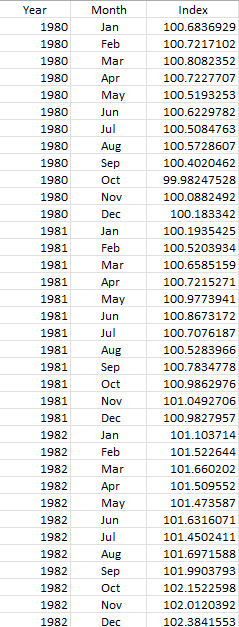
\includegraphics[width=0.5\textwidth]{screenshot019}
	\caption{A Section of the Data Set}
	\label{fig:screenshot019}
\end{figure}

The dataset spans a long period, providing a total of 543 monthly data points of Sri Lanka’s Commodity Net Export Price Index, Individual Commodities Weighted by Ratio of Net Exports to GDP, from January 1980 to March 2025.

IMF provides standardized long-term monthly data based on 45 commodities. These data are consistent, highly reliable, regularly updated in line with IMF’s World Economic Outlook (WEO) cycle, internationally comparable, and widely used in macroeconomic analysis. These properties make the dataset well suited for time series modeling and forecasting using ARIMA.

\setcounter{chapter}{3}

\chapter{Methodology}

\section{Methodology of The Principal Variable}
The principal variable used in this study is the Commodity Net Export Price Index (CNEPI) for Sri Lanka, constructed following the methodology of Spatafora and Tytell (2009) and the International Monetary Fund (IMF) Commodity Terms of Trade Database. The CNEPI shows Sri Lanka's exposure to global commodity price fluctuations by weighting individual commodity prices with their respective ratio of net export to GDP.

The methodology involves four main steps:

\subsection*{1.Commodity Price Data}
Monthly international prices of up to forty-five commodities are obtained from the IMF database, expressed in U.S. dollars.

\subsection*{2.Weighting Scheme}
The monthly weight of each commodity is given by its net export share in GDP:
\[
w_{i,m,y} = \frac{p_{i,m,y} - q_{i,m,y}}{GDP_{m,y}}
\]
where $p_{i,m,y}$ ($q_{i,m,y}$) denotes the exports (imports) value of commodity $i$, in month $m$ year $y$, expressed in US dollars; and $GDP_{m,y}$ denotes the country's nominal GDP in US dollars in month $m$ year $y$.

Using net exports to weight individual commodities ensures that price variations of imported commodities are considered. Commodities for which Sri Lanka is a net exporter are assigned positive weights, while commodities for which it is a net importer are assigned negative weights.

\subsection*{3.Index Construction}
The Commodity Net Export Price Index is obtained as a weighted sum of international commodity prices:
\[
CNEPI_{m,y} = \sum_{i=1}^{N} w_{i,m,y} \times x_{i,m,y}
\]
where $w_{i,m,y}$ is the net export weight of commodity $i$ and $x_{i,m,y}$ is the international price of commodity $i$ at month $m$ year $y$. This ensures that price increases in commodities Sri Lanka imports reduce the index, while price increases in exported commodities raise it.

\subsection*{4.Normalization}
To make it comparable over time, the index is normalized to base year 2010 = 100. A reading above one hundred indicates higher net export-weighted prices relative to the base year and below one hundred readings indicate lower relative prices.


In summary, the CNEPI is built by multiplying each commodity’s net export share of GDP with its international price, so the index directly measures how external price shocks affect the country’s economy.

\section{Research Design}
In this study, the data set was first divided into a training set and a testing set, where 80\% of the observations were used for training and the remaining 20\% for testing. The entire model identification, estimation, and diagnostic checking procedures were carried out using the training set. After selecting candidate ARIMA models, their forecasting performance was evaluated on the testing set to measure out-of-sample accuracy. Finally, the best-performing model was refitted using the full data set, and this refitted model was employed to generate the final forecasts.

\section{Data Analysis Method}
This research is based on the ARIMA model, to analyse and formulate different models to select the best model for forecasting. R statistical software is used.

\section{Statistical Method}
ARIMA, which stands for Auto-Regressive Integrated Moving Average, is a statistical method for analysing and forecasting time series data in economic forecasting (Wikipedia, 2025). It combines three key components: Autoregressive (AR), Integrated (I), and Moving Average (MA).
\begin{itemize}
	\item \textbf{Autoregressive (AR):} This component accounts for the influence of past values of the time series on the current value. It utilizes a linear regression model to predict the current value based on a fixed number of past values ($p$).
	\item \textbf{Integrated (I):} This component deals with non-stationarity in the time series. It employs differencing to erase trends and seasonality, putting the data into a stable form. The degree of differencing necessary is given by $d$.
	\item \textbf{Moving Average (MA):} This component incorporates the impact of prior random errors (shocks) on the current value. It utilizes a linear regression model to forecast the current value based on a fixed number of past errors ($q$).
\end{itemize}

\begin{figure}[h!]
	\centering
	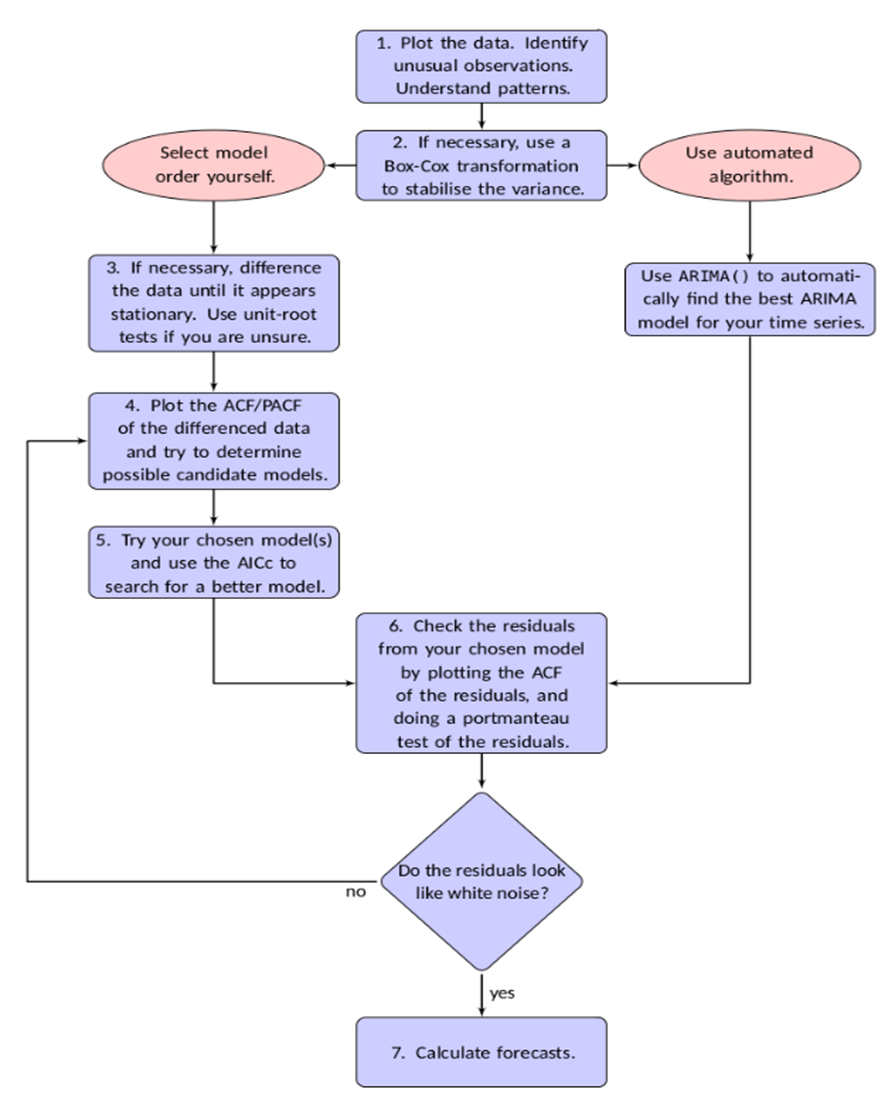
\includegraphics[width=1.0\textwidth]{screenshot020}
	\caption{General process for forecasting using an ARIMA model, Adapted from (Hyndman \& Athanasopoulos, 2021)}
	\label{fig:screenshot020}
\end{figure}

In general, a non-seasonal ARIMA model is expressed as ARIMA($p,d,q$), where $p$ is the number of autoregressive terms, $d$ is the number of non-seasonal differences needed for stationarity, and $q$ is the number of lagged forecast errors in the prediction equation (Poudel et al, 2024).

The ARIMA model with AR order $p$, degree of first differencing $d$, and MA order $q$ is given by the formula:
\[
Y'_t = c + \alpha_1 Y'_{t-1} + \alpha_2 Y'_{t-2} + \cdots + \alpha_p Y'_{t-p} + \beta_1 Z_{t-1} + \beta_2 Z_{t-2} + \cdots + Z_{t-q} + Z_t
\]
where $Y'_t$ is the differenced series.



\subsection{Stationarity Check for the Time Series Data}
The identification step involves analysing the time series data to determine whether it is stationary, where the observations change over a constant mean and a constant variance. If the data are non-stationary, we need to obtain the stationary series using first order differencing (Ghosh, 2017). Additionally, if the series has a strong and consistent seasonal pattern, seasonal differencing will be performed on the data. It is sufficient to apply first-order seasonal differencing in most of the situations (Pallawala and Jayasundara, 2013).

A series, which have no trend, constant variance over time and no periodic fluctuations is defined as a stationary series. For practical purposes, stationarity can usually be determined from a run sequence plot. If the time series is not stationary, it is transformed to stationarity with one of the following techniques:
\begin{enumerate}
	\item If the data shows variation that increases or decreases with the level of the series, then the logarithmic transformation is used. If we denote the original observations as $y_1, \ldots, y_t$ and the transformed observations as $W_1, \ldots, W_t$, the transformation will be $W_t = \log(y_t)$. Following this process, the variance of the original series will be turned into a constant.
	\item The first-order difference (non-seasonal difference) of a time series is the series of changes from one period to the next. If $Y_t$ denotes the value of the time series $Y$ at period $t$, then the first difference of $Y$ at period $t$ ($\Delta Y_t$) is equal to $Y_t - Y_{t-1}$. If the first difference (lag 1 difference) of $Y$ is stationary and not correlated, the process ($Y_t$) is defined as a random walk process, which is the same as the white noise process. It helps to stabilize the mean of a time series.
	\item A seasonal difference of the time series is defined to be the difference between an observation and the corresponding observation from the previous season. With $m$ seasons, the equation for the seasonal differencing is defined as:
	\[
	\Delta_m Y_t = Y_t - Y_{t-m}
	\]
\end{enumerate}

To further prove the stationarity of the time series apart from the ACF and PACF, the Augmented Dickey Fuller (ADF) test is used. 
	\begin{quote}
	H$_0$: The series has a unit root (non-stationary) \\
	H$_1$: The series is stationary
\end{quote}
 The $p$-value obtained should be less than the significance level ($\alpha = 0.05$) to reject the null hypothesis, thereby proving the series is stationary (Mesike et al., 2014).

\subsection{Model Identification}
Once stationarity has been achieved, this can be accomplished by looking at the time series data's autocorrelation function (ACF) and partial autocorrelation function (PACF). 
\begin{itemize}
	\item A sharp cutoff in the PACF with gradual decay in the ACF suggests an AR($p$) process.
	\item A sharp cutoff in the ACF with gradual decay in the PACF suggests an MA($q$) process.
	\item Mixed patterns suggest a combination ARMA($p,q$).
\end{itemize}
The number of significant lags provides an initial estimate of $p$ and $q$. The parameter $d$ tells how many times differencing is applied to make a non-stationary series into a stationary one.

\subsection{Model Estimation}
Upon determining the order ($p,d,q$), it is necessary to estimate the parameters $c, \alpha_1, \ldots, \alpha_p, \beta_1, \ldots, \beta_q$ to identify the appropriate model. The model's predicted parameter values were determined in relation to each coefficient's $p$-value using the $z$-test of coefficients. Since the significance value ($\alpha = 0.05$) was greater than the $p$-value, the null hypothesis that none of the model's parameters are significant was rejected.

\subsection{Model Evaluation Methods }
In this study, the best fitting ARIMA model for time series forecasting was estimated using the Bayesian Information Criterion (BIC) and the Akaike Information Criterion (AIC). Both metrics aid in preventing overfitting, and the model with the lowest AIC or BIC value is typically regarded as the most suitable (Akaike et al, 1974).

\subsection{Diagnostic Checking}
After the ARIMA model has been estimated, it is crucial to verify that the residuals are white noise and that the model fits well (Poudel et al, 2024).

To check the validity of the assumption that the residuals are white noise, the Ljung-Box test was used:

\begin{quote}
	H$_0$: Residuals are independent \\
	H$_1$: Residuals are not independent
\end{quote}

The study also checked the normality of the residuals using the Shapiro-Wilk normality test with significance level $\alpha = 0.05$:

\begin{quote}
	H$_0$: The residuals are normally distributed \\
	H$_1$: The residuals are not normally distributed
\end{quote}


\subsection{Forecasting Values in the Test Set}
Once the ARIMA model has been estimated and checked, it can be used to forecast the values in the testing set.

\subsection{Forecasting Evaluation Methods}
To evaluate forecasting accuracy, Root Mean Squared Error (RMSE), Mean Absolute Scaled Error (MASE), Mean Absolute Percentage Error (MAPE) and Mean Absolute Error (MAE) were used in the study. By comparing these measures, the study identifies the best-performing model, giving more importance to forecasting accuracy.

\subsection{Forecasting Future Values}
As the final step, the forecasting was done using the entire data set with the chosen ARIMA model for the next 12 months.


% Number subsections as 6.1, 6.2, ...
\setcounter{chapter}{4} % So next chapter becomes Chapter 6

	\chapter{Analysis of Data} % This will be Chapter 6
	
	\section{Preliminary (Exploratory) Analysis}
	
	According to Figure~\ref{fig:screenshot001}, some trend patterns can be identified in the time series. Until 1998, it shows an approximate upward trend in the Commodity Net Export Price Index over time. From that point until 2008, there is a clear downward trend. After that, a clear trend is not identifiable.
	
	
	\begin{figure}[h!]
		\centering
		\includegraphics[width=0.8\textwidth]{"screenshot001"}
		\caption{Time Series Plot of Commodity Net Export Price Index from 1980 M1 to 2025 M3 (Original Data Set)}
		\label{fig:screenshot001}
	\end{figure}
	
	
	In time series analysis, the original data set should first be split into two sections: a \textbf{training set} and a \textbf{test set}. The model will be fitted using the training set, and then its performance will be evaluated using the test set. Figure~\ref{fig:screenshot002} shows the time series plot of the Commodity Net Export Price Index based on the training set. From this point until a suitable model is fitted, the entire analysis will be performed based on the training set.
	
	
	\begin{figure}[h!]
		\centering
		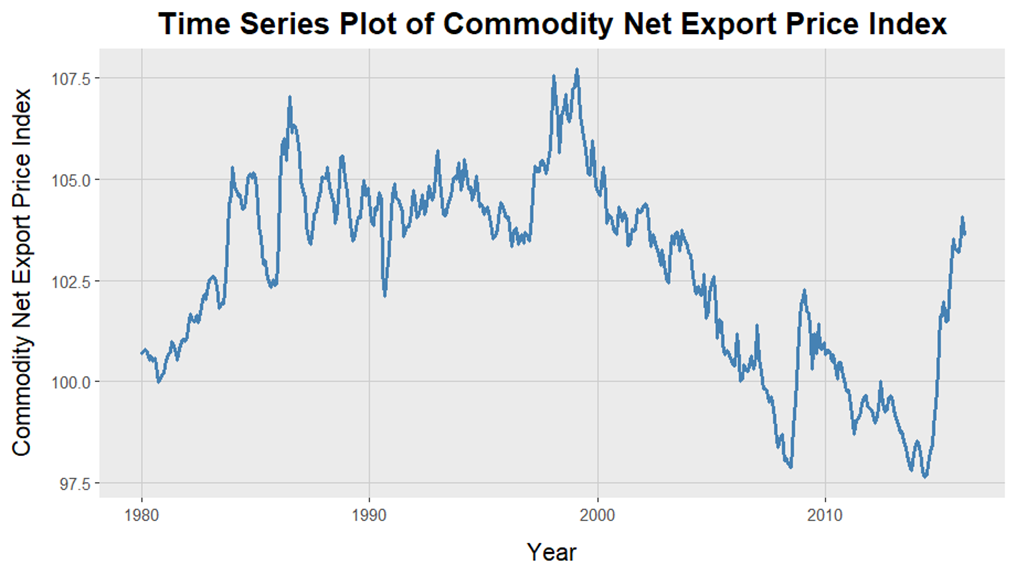
\includegraphics[width=0.8\textwidth]{screenshot002}
		\caption{Time Series Plot of Commodity Net Export Price Index from 1980 M1 to 2016 M2 (For Training Set)}
		\label{fig:screenshot002}
	\end{figure}
	
	
	Figure~\ref{fig:screenshot002} also suggests some trend patterns over time. However, it does not show a clear seasonal pattern in the Commodity Net Export Price Index data. Figures~\ref{fig:screenshot003} and \ref{fig:screenshot004} also confirm that there is no significant seasonal variation.
	
	
	\begin{figure}[h!]
		\centering
		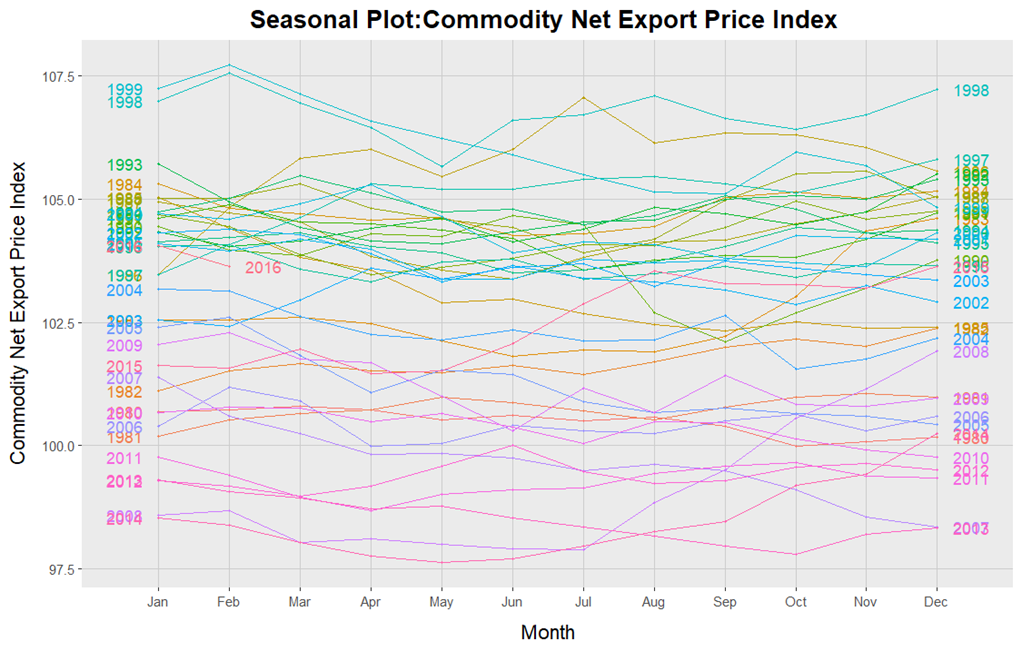
\includegraphics[width=0.8\textwidth]{screenshot003}
		\caption{Seasonal Plot of Commodity Net Export Price Index}
		\label{fig:screenshot003}
	\end{figure}
	
	
	Furthermore, the time series plot shows some sudden changes, particularly the big drop in 2008/2009. Otherwise, there are no unusual variations in the time series plot. This suggests that a Box–Cox transformation is not needed to stabilise the variance.
	
	
	\begin{figure}[h!]
		\centering
		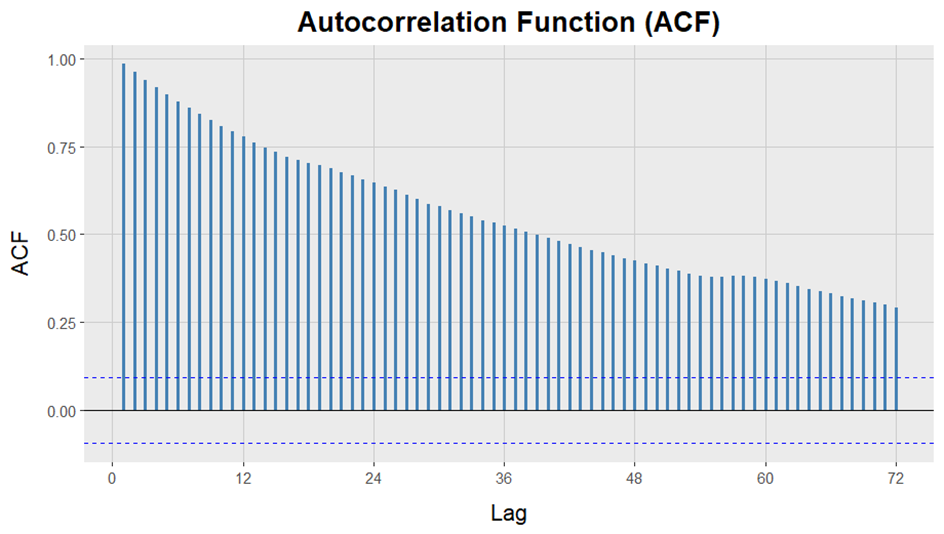
\includegraphics[width=0.8\textwidth]{screenshot004}
		\caption{ACF Plot of the Commodity Net Export Price Index}
		\label{fig:screenshot004}
	\end{figure}
	
	
	\section{Test for Stationarity}
	
	The presence of a trend pattern in the time series plot (Figure~\ref{fig:screenshot002}) provides a rough idea that the time series is not stationary. The Auto Correlation Function (ACF) plot (Figure~\ref{fig:screenshot004}) also confirms this. If a time series contains a trend, then the values of the ACF will not decay to zero except for very large values of the lag.  
	
	However, the \textit{Augmented Dickey–Fuller (ADF) Test} is a standard statistical test for checking stationarity. The ADF test was conducted under $\alpha = 0.05$. The results are summarised in Table~\ref{tab:adf}.
	
	
	\begin{table}[h!]
		\centering
		\caption{ADF Test Result on Commodity Net Export Price Index}
		\label{tab:adf}
		\begin{tabular}{l c c c c}
			\toprule
			& \textbf{Data} & \textbf{Test Statistic} & \textbf{Lag Order} & \textbf{p-value} \\
			\midrule
			ADF Test Result & train\_ts & -2.5992 & 7 & 0.3243 \\
			\bottomrule
		\end{tabular}
	\end{table}
	
	According to Table~\ref{tab:adf}, the null hypothesis of the existence of a unit root cannot be rejected at the 5\% level of significance since the p-value is 0.3243 $>$ 0.05. As the original time series does not reveal any seasonal pattern, non-seasonal differencing is appropriate to obtain a stationary series. Hence, first-order differencing was applied to the original series.
	
	
	\begin{figure}[h!]
		\centering
		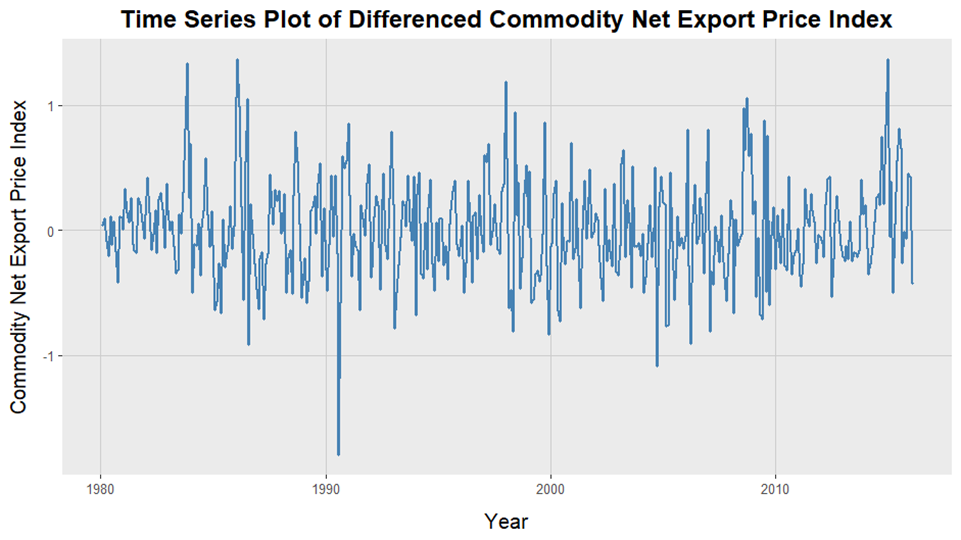
\includegraphics[width=0.8\textwidth]{screenshot006}
		\caption{Time Series Plot of Differenced Commodity Net Export Price Index from 1980 M1 to 2016 M2}
		\label{fig:screenshot006}
	\end{figure}
	
	
	As shown in Figure~\ref{fig:screenshot006}, the differenced series does not appear to have a trend over time, though there are some fluctuations. However, this is not strong evidence of violation of constant variance. Therefore, the differenced series provides a rough idea of satisfying the stationarity assumption.  
	
	The ACF plot of the differenced Commodity Net Export Price Index (Figure~\ref{fig:screenshot009}) also supports this conclusion. Some significant lags can be observed after the cutoff point; however, since they are far from the cutoff, they can be considered negligible (Nelson, 1998). To obtain an exact conclusion about stationarity, the ADF test was also applied to the differenced series.
	
	
	\begin{table}[h!]
		\centering
		\caption{ADF Test Result on Differenced Commodity Net Export Price Index}
		\label{tab:adfdiff}
		\begin{tabular}{l c c c c}
			\toprule
			& \textbf{Data} & \textbf{Test Statistic} & \textbf{Lag Order} & \textbf{p-value} \\
			\midrule
			ADF Test Result & train\_ts\_diff & -7.6126 & 7 & 0.01 \\
			\bottomrule
		\end{tabular}
	\end{table}
	
	
	As Table~\ref{tab:adfdiff} provided, concerning the Commodity Net Export Price Index, p-value is 0.0100 $<$ 0.05. Hence, there is strong evidence that the sequence is stationary after differencing operations at 95\% confidence level.
	
	\section{Choosing and Fitting Models}
	
	\begin{figure}[h!]
		\centering
		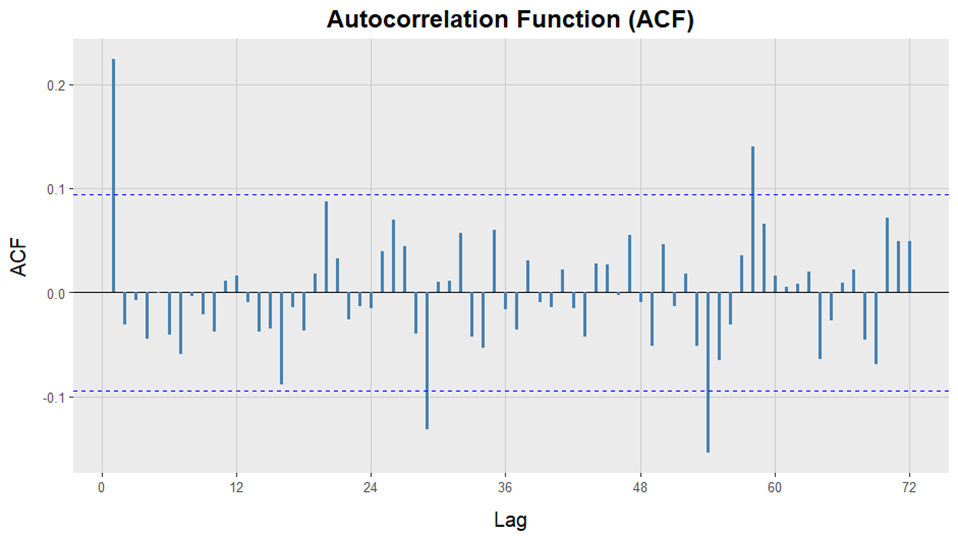
\includegraphics[width=0.8\textwidth]{screenshot009}
		\caption{ACF Plot of Differenced Commodity Net Export Price Index}
		\label{fig:screenshot009}
	\end{figure}
	
	\begin{figure}[h!]
		\centering
		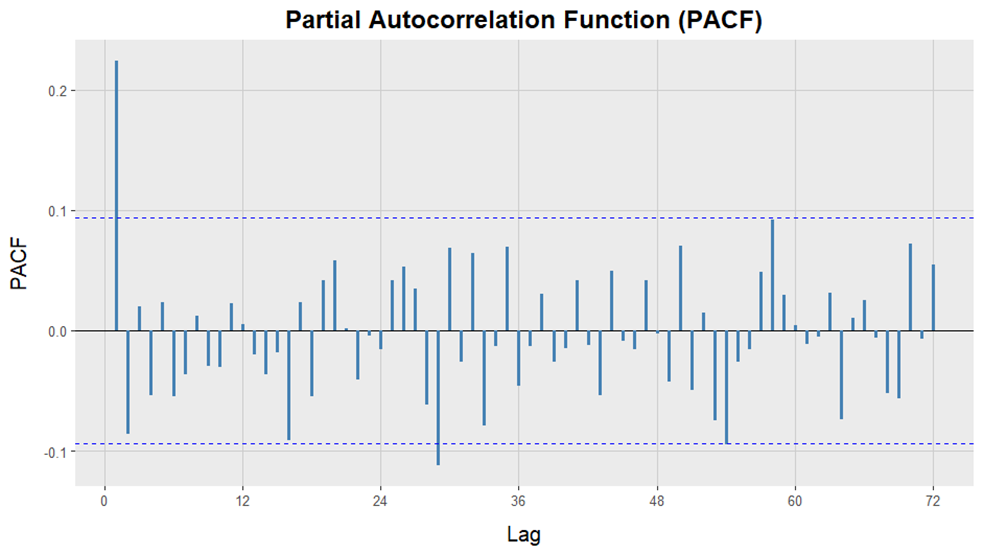
\includegraphics[width=0.8\textwidth]{screenshot011}
		\caption{PACF Plot of Differenced Commodity Net Export Price Index}
		\label{fig:screenshot011}
	\end{figure}
	
	The ACF and PACF plots shown in Figure~\ref{fig:screenshot009} and Figure~\ref{fig:screenshot011} do not reveal any obvious pattern, such as exponential decay or sinusoidal behavior. However, according to Hyndman (2024), when both the order of the autoregressive part ($p$) and the order of the moving average part ($q$) are positive, the ACF and PACF are not particularly useful in determining suitable values of $p$ and $q$. In this case, identifying only the cutoff points of the PACF and ACF as $p$ and $q$, an initial candidate model can be specified. That model is ARIMA($1,1,1$), since the degree of first differencing involved ($d$) is 1. This candidate model was then compared with several alternative models, as summarized in Table~\ref{mod:eva}.
	
	\section{Model Evaluation}
	
	\begin{table}[htbp]
		\centering
		\caption{Model Evaluation}
		\label{mod:eva}
		\resizebox{\textwidth}{!}{%
			\begin{tabular}{l c c c c c c c c c c }
				\hline
				ARIMA & AIC & BIC & \multicolumn{4}{c}{Training set} & \multicolumn{4}{c}{Testing Set}  \\
				\cline{4-7} \cline{8-11}
				& & & RMSE & MAE & MAPE & MASE & RMSE & MAE & MAPE & MASE   \\
				\hline
				(1,1,1) & 425.39 & 441.67 & 0.3913593 & 0.3007561 & 0.29199 & 0.259333 & 3.6540172 & 3.2924804 & 3.295765 & 2.839008  \\
				(0,1,1) & 424.27\textcolor{red}{*} & 436.48\textcolor{red}{*} & 0.3917608 & 0.3006242 & 0.2918535 & 0.2592192 & 3.6289076 & 3.2657318 & 3.2691366 & 2.8159431 \\
				(1,1,0) & 427.50 & 439.71 & 0.3932331 & 0.3013476 & 0.2925516 & 0.259843 & 3.6310129 & 3.2688683 & 3.2722342 & 2.818648  \\
				(0,1,0) & 447.85 & 455.99 & 0.4035348 & 0.3099021 & 0.3008729 & 0.2672193 & 3.7629143 & 3.4088608 & 3.4116004 & 2.9393589  \\
				(2,1,2) & 428.98 & 453.40 & 0.3911704 & 0.3004418 & 0.2916704 & 0.259062 & 3.6155956 & 3.2572448 & 3.2605298 & 2.808625 \\
				(2,1,1) & 427.06 & 447.42 & 0.3912109 & 0.3005401 & 0.2917733 & 0.2591468 & 3.6549473 & 3.2936124 & 3.2968879 & 2.8399837 \\
				(1,1,2) & 426.85 & 447.20 & 0.3911103 & 0.3002488 & 0.2914718 & 0.2588956 & 3.6457367 & 3.2832724 & 3.2866092 & 2.8310678  \\
				(2,1,0) & 426.23 & 442.52 & 0.3917452 & 0.3009799 & 0.2922077 & 0.259526 & 3.6344585 & 3.2717385 & 3.2751138 & 2.821122  \\
				(0,1,2) & 425.54 & 441.82 & 0.3914286 & 0.3007543 & 0.2919874 & 0.2593314 & 3.6463450 & 3.2844741 & 3.2877902 & 2.832104  \\
				(1,1,3) & 428.78 & 453.20 & 0.3910763 & 0.3003346 & 0.2915573 & 0.2589696 & 3.6409492 & 3.2793366 & 3.2826589 & 2.8276741  \\
				(3,1,1) & 428.71 & 453.13 & 0.3910444 & 0.3004462 & 0.2916654 & 0.2590658 & 3.6414794 & 3.2792242 & 3.2825658 & 2.8275772  \\
				(3,1,2) & 428.68 & 457.17 & 0.3901061 & 0.2999112 & 0.2912139 & 0.2586045 & 2.6688530 & 2.2918109 & 2.2974849 & 1.9761601  \\
				(2,1,3) & 428.24 & 456.74 & 0.3891667\textcolor{red}{*} & 0.2986667\textcolor{red}{*} & 0.2900096\textcolor{red}{*} & 0.2575314\textcolor{red}{*} & 2.3036126\textcolor{red}{*} & 2.0122170\textcolor{red}{*} & 2.0155581\textcolor{red}{*} & 1.7350746\textcolor{red}{*}  \\
				(3,1,3) & 430.67 & 463.24 & 0.3901037 & 0.2998439 & 0.2911510 & 0.2585464 & 2.6887665 & 2.3091039 & 2.3148320 & 1.9910714  \\
				(3,1,0) & 428.07 & 448.42 & 0.3916690 & 0.3008233 & 0.2920518 & 0.2593909 & 3.6427020 & 3.2804568 & 3.2837948 & 2.8286400  \\
				\hline
			\end{tabular}%
		}
	\end{table}
	
	
	Compared with several models in Table~\ref{mod:eva}, the ARIMA(0,1,1) model has the smallest Akaike’s Information Criterion (AIC) and Bayesian Information Criterion (BIC). Therefore, it can be considered that the ARIMA(0,1,1) model has the best fitting effect. 
	
	However, the ARIMA(2,1,3) model has the smallest RMSE, MAE, MAPE, and MASE for the training set, and the smallest RMSE, MAE, MAPE and MASE for the test set. Hence, both in-sample forecasting accuracy and out-of-sample forecasting accuracy are high in ARIMA(2,1,3). Furthermore, AIC and BIC are not much higher than those of ARIMA(0,1,1). Since our main objective is also to build a parsimonious time series model that produces accurate forecasts, ARIMA(2,1,3) was chosen. 
	
	At this point, the model formula can be obtained as (Table~\ref{mod:para}):
	\[
	Y'_t = -0.0022 + 0.1130\,Y'_{t-1} + 0.8485\,Y'_{t-2} + 0.1279\,Z_{t-1} - 0.9217\,Z_{t-2} - 0.2062\,Z_{t-3} + Z_t
	\]
	where $Y'_t = Y_t - Y_{t-1}$
		
	\[
	\resizebox{\textwidth}{!}{$
		Y_t = -0.0022 + B\,Y_{t} + 0.1130(1-B)B\,Y_{t} + 0.8485(1-B)B^{2}Y_{t}
		+ 0.1279\,B\,Z_{t} - 0.9217\,B^2\,Z_{t} - 0.2062\,B^3\,Z_{t} + Z_t
		$}
	\]

	
	\begin{table}[htbp]
		\centering
		\caption{ARIMA(2,1,3) Model Parameter List}
		\label{mod:para}
		\begin{tabular}{l c c c}
			\hline
			Item & Signe & Coeff. & SE \\
			\hline
			Constant & $c$ & -0.0022 & 0.0073 \\
			AR & $\alpha_1$ & 0.1130 & 0.1436 \\
			& $\alpha_2$ & 0.8485 & 0.1394 \\
			MA & $\beta_1$ & 0.1279 & 0.1553 \\
			& $\beta_2$ & -0.9217 & 0.0915 \\
			& $\beta_3$ & -0.2062 & 0.0751 \\
			\hline
		\end{tabular}
	\end{table}
	
	
	\section{Residual Diagnostics}
	
	The Box-Ljung test was applied to test for the independence of the residuals.
	
	
	\begin{table}[h!]
		\centering
		\caption{Box-Ljung Test on Residuals}
		\label{tab:res}
		\begin{tabular}{l c c c c}
			\toprule
			& \textbf{Data} & \textbf{X-squared} & \textbf{df} & \textbf{p-value} \\
			\midrule
			Box-Ljung Test Result & residuals(model13) & 10.782 & 24 & 0.9905 \\
			\bottomrule
		\end{tabular}
	\end{table}
	
	
	In Table~\ref{tab:res}, the $p$-value is 0.9905 $> 0.05$. Therefore, $H_0$ will not be rejected at the 5\% significance level. Hence, there is sufficient evidence to conclude that the residuals are independent at the 95\% confidence level. Otherwise, the residuals are considered white noise.
	
	
	\begin{table}[h!]
		\centering
		\caption{Shapiro-Wilk Normality Test on Residuals}
		\label{tab:normality}
		\begin{tabular}{l c c c c}
			\toprule
			& \textbf{Data} & \textbf{W} & \textbf{p-value} \\
			\midrule
			Shapiro-Wilk Test Result & residuals(model13) & 0.98797 & 0.001206 \\
			\bottomrule
		\end{tabular}
	\end{table}
	
	According to Table~\ref{tab:normality}, the null hypothesis of the Shapiro-Wilk Test for normality is rejected at $\alpha = 0.05$ since $p$-value $< 0.05$, i.e., residuals are not normally distributed. But this is not a major concern for forecasting accuracy in ARIMA models. This may be a serious problem in statistical inference, but in the forecasting context, independence is the most serious assumption (Yüreki et al., 2005).
	
	\begin{figure}[h!]
		\centering
		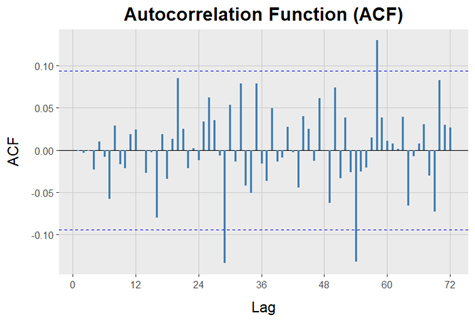
\includegraphics[width=0.45\textwidth]{screenshot013}
		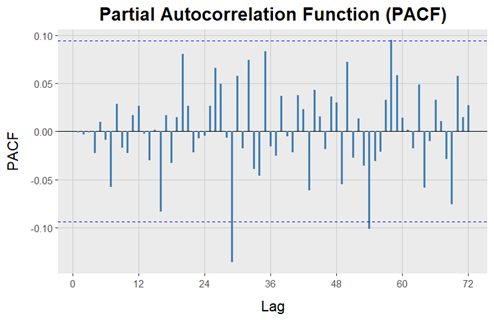
\includegraphics[width=0.45\textwidth]{screenshot014}
		\caption{ACF Plot and PACF Plot of Residuals}
		\label{fig:screenshot014}
	\end{figure}
	
	Figures~\ref{fig:screenshot014} show that most spikes are inside the confidence bounds. Although there are significant lags at higher orders, they can be considered negligible. Almost all autocorrelations and partial autocorrelations are approximately zero. Therefore, the series of residuals is stationary and follows a white noise process.
	
	\begin{figure}[h!]
		\centering
		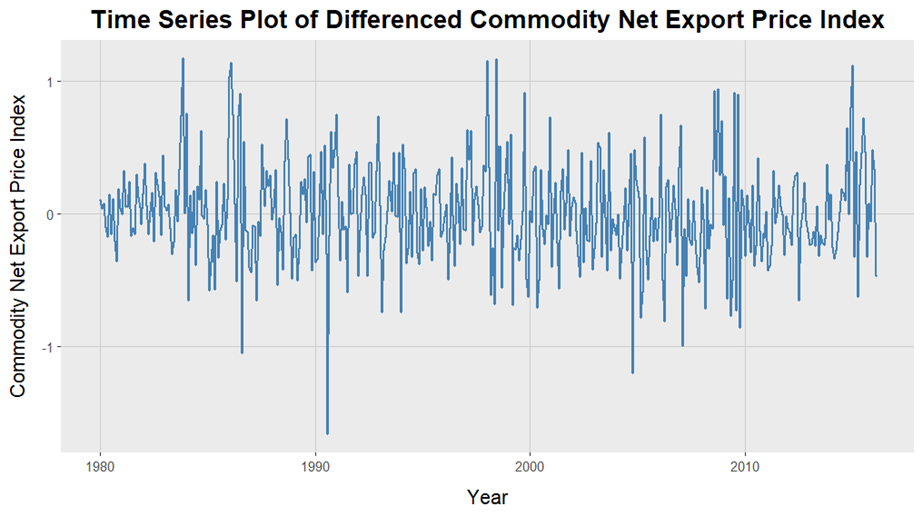
\includegraphics[width=0.7\textwidth]{screenshot015}
		\caption{Time Series Plot of Residuals}
		\label{fig:screenshot015}
	\end{figure}
	
	The time series plot of residuals (Figure~\ref{fig:screenshot015}) is approximately symmetric around the zero baseline without any unusual structure. Hence, it indicates that the zeroth mean assumption and the constant variance assumption are satisfied. For these reasons, the ARIMA(2,1,3) model is considered adequate.
	
	
	\section{Forecasting Future Values}
	\label{sec:forecasting}
	
	After the diagnostic checking had been completed successfully, the Commodity Net Export Price Index could be forecasted using the ARIMA(2,1,3) model. Table~\ref{tab:forecast_values} summarises the results of forecasting the Commodity Net Export Price Index over the period 2025M4 to 2026M3.
	
	According to Figure~\ref{fig:screenshot017}, the fitting degree of the numerical model is high and very close to the distribution of the true values. Hence, using ARIMA(2,1,3) to forecast the Commodity Net Export Price Index is reliable.
	
	\begin{table}[h!]
		\centering
		\caption{Forecasted Values of the Commodity Net Export Price Index}
		\label{tab:forecast_values}
		\begin{tabular}{l l r}
			\hline
			Year & Month & Forecasted Value \\
			\hline
			2025 & April      & 100.8114 \\
			2025 & May        & 100.8102 \\
			2025 & June       & 100.8325 \\
			2025 & July       & 100.8339 \\
			2025 & August     & 100.8529 \\
			2025 & September  & 100.8561 \\
			2025 & October    & 100.8725 \\
			2025 & November   & 100.8770 \\
			2025 & December   & 100.8913 \\
			2026 & January    & 100.8967 \\
			2026 & February   & 100.9094 \\
			2026 & March      & 100.9153 \\
			\hline
		\end{tabular}
	\end{table}
	
	According to Table~\ref{tab:forecast_values}, the forecasted values of the Commodity Net Export Price Index within the next 12 months show an increasing trend.
	
	\begin{figure}[h!]
		\centering
		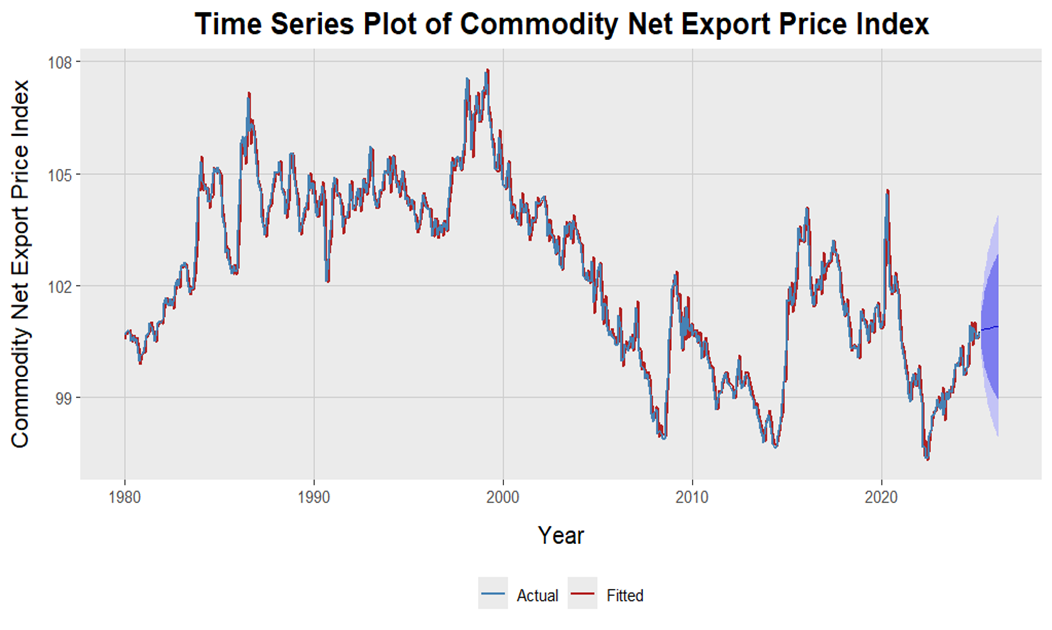
\includegraphics[width=1.1\textwidth]{screenshot017}
		\caption{Fitting and Prediction of the Commodity Net Export Price Index}
		\label{fig:screenshot017}
	\end{figure}
	
	\setcounter{chapter}{5} % So next chapter becomes Chapter 6
	
		
		\chapter{Discussion }
		
		This study focused on analyzing Net Export Price Index for Sri Lanka form 1980 January to 2025 March in the aim of identifying suitable forecasting models and interpret economic pattern of the observed values. This section interprets the results obtained from time series decomposition, stationary testing autocorrelation diagnostics, ARIMA model estimation and forecasting evaluation. This report evaluated ARIMA based forecasting approaches using training and testing framework.
		
		The time series plot of full dataset (Figure~\ref{fig:screenshot001})  reveals that the Commodity Net Export Price Index fluctuates around a long run mean close to 102, this gives us an idea that it is consistent with long term stability. But we can also observe that the data points fluctuated by several periods which corresponds to both global and domestic economic crisis. We can see drastic decrease in the index in the year of 2008 because of the global financial crisis or (the panic of 2008 - major worldwide financial crisis centered in the United States). Second major off trend is in 2020 due to covid 19 pandemic, there we can see sudden upward push in index, but it doesn’t keep as it is, next year it collapsed down. Third, most recent year (2022), the domestic economic crisis falls behinds and index fall to its lowest levels in decades. This was not mainly on global pressure but also due to internal imbalance due to shortage of foreign exchange, debt repayment pressure and currency depreciation. As we can see after several sharp declines, the index gradually corrected to the way of long run level.
		
		To assess time series characteristics, the Augmented Dickey-Fuller (ADF) test was applied to full data set (Table~\ref{tab:adf}). This test confirmed that the Commodity Net Export Price Index is nonstationary, as the null hypothesis of the existence of a unit root could not rejected. We can say that it indicates the presence of Stochastic trends, which is consistent with the long-term behavior of indexes. However, after applying first differencing the ADF test (Table~\ref{tab:adfdiff}) strongly rejected the null hypothesis. This implies that the index is stationary at lag (1), that its first differencing is stable. This confirms the need of differencing method before applying forecasting models.
		
		The autocorrelation function (ACF) (Figure~\ref{fig:screenshot004}) and partial autocorrelation function (PACF) were analyzed to gain insight into the short run dynamics of the series. For the undifferenced series, the ACF displayed a slow and gradual decay, which is typical of non-stationary data. This further confirmed the need for differencing. After differenced, the ACF (Figure~\ref{fig:screenshot009}) exhibited a sharp spike at lag (1), while the PACF (Figure ~\ref{fig:screenshot011}) cut of at 1st lag. 
		
		This pattern is strongly indicative of an ARIMA structure of the form ARIMA (1,1,1,). The spike in the ACF suggests the presence of moving average dynamics, while the PACF cut off at lag (1) indicates autoregressive dependence. These diagnostic identification of low order ARIMA models suitable for underlying structure of index.
		
		Fifteen number of ARIMA models was estimated on the training data set covering 1980 January to 2016 February (Table~\ref{mod:eva}). These models include simple specification such as ARIMA (1,1,1), A (0,1,1), A (0,1,0) and more complex higher order ARIMA model like A(3,1,2), A(3,1,3). Considering Akaike’s Information Criteria (AIC) and Bayesian Information Criterion (BIC) ARIMA (0,1,1) model has smallest. Therefore, we can consider that ARIMA (0,1,1) has the best fitting value. But smallest RMSE, MAE, MAPE and MASE for the training set and the smallest RMSE, MAE, MAPE and MASE for the test set is fit with ARIMA (2,1,3). Mentioning that our main objective is to build a parsimonious time series model to have accurate forecast measures, ARIMA (2,1,3) was chosen. The model formula can be obtained as in Table~\ref{mod:para}.
		
		Residual diagnostics confirmed the adequacy of the model. The Box Ljung test (Table~\ref{tab:res}) provide string evidence that the residuals are uncorrelated (p value = 0.9905). The Shapiro-Wilk test (Table~\ref{tab:normality}) suggested that the residuals deviate from normality. Here, in forecasting it is not concern as major issue since independence rather than strict normality is the critical assumption in ARIMA modeling. The ACF and PACF plots of the residuals indicated that almost all autocorrelations and partial autocorrelations were within confidence bounds, while the residual time series plot showed symmetry around zero with no visible patterns. Together, these diagnostics confirmed that the ARIMA (2,1,3) model is statistically adequate.
		
		Finally, the model was used to generate forecasts for the Commodity Net Export Price Index for the period 2025 April to 2026 March. The forecasts suggest a gradual upward trend, with values rising from 100.81 in April 2025 to 100.92 by March 2026. This indicates a modest recovery and stabilization of Sri Lanka’s net export competitiveness soon. The forecast plot (Figure~\ref{fig:screenshot017}) further illustrates that the fitted values closely track the observed series, reinforcing the reliability of the model for short term forecasting.
		
		\section{Limitations and Future Research}
		The index used in the study is only for commodities and does not include growing shares of the services provided in Sri Lanka’s trade. For examples tourism, IT services these should be added to the future indices in order to have a clear picture of the economy of Sri Lanka. ARIMA rely only on the past values of the index and it does not include explanatory variables such as exchange rates, interest rate which could further accurately represent the real situation of economy. Therefore, future researchers can extend this study using models such as ARIMAX or VAR. Moreover, the study could be enhanced to explore machine learning approaches, which can provide a valuable next step for improving forecasting accuracy.
		
		\setcounter{chapter}{6}
		
			\chapter{Conclusion}
		
		\section{Main Findings}
		This study successfully found the best model to forecast Sri Lanka's Commodity Net Export Price Index. 
		The ARIMA(2,1,3) model was chosen as the most suitable one, with the equation: 
		\[
		\resizebox{\textwidth}{!}{$
		Y_t = -0.0022 + B\,Y_{t} + 0.1130(1-B)B\,Y_{t} + 0.8485(1-B)B^{2}Y_{t}
		+ 0.1279\,B\,Z_{t} - 0.9217\,B^2\,Z_{t} - 0.2062\,B^3\,Z_{t} + Z_t
		$}
		\]
		This simple model met the main goal of building a parsimonious statistical model to produce accurate forecasts and completed all the smaller objectives too. 
		The model showed the best results compared to 14 other models, with the lowest error rates. 
		The residual tests proved the model works correctly (Box-Ljung test $p$-value = 0.9905). 
		The forecasting results show good news --- the values will increase from 100.81 in April 2025 to 100.92 in March 2026, meaning Sri Lanka's net export position is getting better.
		
		\section{Contribution to the Literature}
		This research fills an important gap because no one has studied this specific index for Sri Lanka before. 
		Earlier studies only looked at single export products like tea, coconut, and pepper, but this research looks at the whole picture of Sri Lanka's trade position. 
		The study shows that simple ARIMA models still work well for predicting complex economic numbers, even during difficult times like Sri Lanka's recent economic problems. 
		Other researchers studying developing countries can use the same methods from this study to forecast similar trade indicators.
		
		\section{Implications}
		The positive forecasting trend is good news for Sri Lanka's economic recovery, showing that the country's export competitiveness is slowly improving after the 2022 crisis. 
		Policymakers can see that their current trade policies are helping, but they need to keep watching because world economic changes can still affect the index. 
		Export businesses can use these forecasts to make better plans since the increasing trend shows Sri Lanka's products are becoming more competitive in world markets. 
		Researchers in other developing countries can also use these methods to study their own trade indicators and help their governments make better economic decisions.
	
	
\clearpage
\chapter*{Appendix}
\addcontentsline{toc}{chapter}{Appendix}
\pagestyle{empty}

\section*{A. Appendix to Chapter 03}
\addcontentsline{toc}{section}{A. Appendix to Chapter 03}
This appendix contains a link to our Excel file with the complete data set stored on OneDrive.

\begin{tcolorbox}[colback=gray!10, colframe=black, width=0.95\linewidth, sharp corners, boxrule=0.8mm, title={\faFileExcel~Dataset Preview}]
	\centering
	Click the link below to open or download the file:
	
	\href{https://1drv.ms/x/c/5052e625e7f51e50/Efz9E37GlIZKrV8SN2bB7dYBz1Fz8i85WacAgvEQRouHsw?e=yonf3T&nav=MTVfezNGMEJENEU5LUQ0N0ItNDFBQy1BNEEyLTYzNkBEQTFENkE1Q30}{\textbf{\textcolor{black}{Download Dataset.xlsx}}}
\end{tcolorbox}


\section*{B. Appendix to Chapter 05}
\addcontentsline{toc}{section}{B. Appendix to Chapter 05}
This appendix contains a link to our R script with the full analysis stored on OneDrive.


\begin{tcolorbox}[colback=gray!10, colframe=black, width=0.95\linewidth, sharp corners, boxrule=0.8mm, title={\faFileCode~R Script Preview}]
	\centering
	Click the link below to open or download the file:
	
	\href{https://1drv.ms/u/c/5052e625e7f51e50/EcsEFY5C1YRDq0fjz8jZahsBZrp3K-bhtD9727I739Jcrg?e=LCo3bv}{\textbf{\textcolor{black}{Download Estimating CNEPI.R}}}
\end{tcolorbox}


		
	
	% ===========================
	% References Section (Manual)
	% ===========================
\clearpage
	\chapter*{References}
	\addcontentsline{toc}{chapter}{References}
	\pagestyle{empty}
	\begin{enumerate}
		\item Peltonen, T. A., Skala, M., Santos Rivera, A., and Pula, G., 2008. Imports and
		profitability in the euro area manufacturing sector: The role of emerging market
		economies.
		
		\item Hutchison, M. and Singh, N., 1992. Exports, non-exports and externalities: a Granger
		causality approach.
		
		\item Fung, K.C., 1994. Empirical Studies of Strategic Trade Policy.
		
		\item Toaca, Z., Staver, L., Stratan, A., Lopotenco, V. and Cociug, V., 2025. Forecasting
		Moldova’s monthly exports using autoregressive models with seasonal dummies. \textit{Cogent
			Business \& Management}, 12(1), p.2519988.
		
		\item Wan, X., Kazmi, S. A. A., \& Wong, C. Y., 2022. Manufacturing, exports, and sustainable
		growth: Evidence from developing countries. \textit{Sustainability}, 14(3), 1646.
		\url{https://doi.org/10.3390/su14031646}
		
		\item Dridi, J. and Zieschang, K., 2004. Export and import price indices. \textit{IMF Staff
			Papers}, 51(1), pp.157-194.
		
		\item Okyere, I. and Jilu, L., 2020. The impact of export and import to economic growth of
		Ghana. \textit{European Journal of Business and Management}, 12(21), pp.130-138.
		
		\item Akalpler, E. and Shamadeen, B., 2017. The Role of Net Export on Economic Growth
		in United States of America. \textit{Journal of Applied Economic Sciences}, 12(3).
		
		\item Malhotra, N. and Kumari, D., 2016. Determinants of exports in major Asian
		economies. \textit{Journal of International Economics}, 7(1), p.94.
		
		\item Liu, Z., Zhu, Z., Gao, J., \& Xu, C., 2021. Forecast methods for time series data: A
		survey. \textit{IEEE Access}, 9, 91896–91912. \url{https://doi.org/10.1109/ACCESS.2021.3091162}
		
		\item Ghauri, S.P., Ahmed, R.R., Streimikiene, D. and Streimikis, J., 2020. Forecasting exports
		and imports by using autoregressive (AR) with seasonal dummies and Box-Jenkins
		approaches: A case of Pakistan. \textit{Inžinerinė ekonomika}, 31(3), pp.291-301.
		
		\item Jammeh, L. B., Guobadia, E. K., \& Ugoh, C. I., 2023. Exponential smoothing state space
		innovation model for forecasting export commodity price index in Nigeria. \textit{Development}, 6(4),
		74–84.
		
		\item Ramos, M. C., and Ativo, R. G., 2023. Forecasting Agricultural Commodity Prices Using
		ARIMA Model. \textit{International Journal of Research Publication and Reviews}, 4(1), 1983-1993.
		
		\item Frankel, J.A., 2005. Peg the export price index: A proposed monetary regime for small
		countries. \textit{Journal of Policy Modeling}, 27(4), pp.495-508.
		
		\item Lehmann, R., 2021. Forecasting exports across Europe: What are the superior survey
		indicators?. \textit{Empirical Economics}, 60(5), pp.2429-2453.
		
		\item Grimme, C. and Lehmann, R., 2019. The ifo Export Climate–a leading indicator to
		forecast German export growth. \textit{CESifo Forum} (Vol. 20, No. 04, pp. 36-42). München:
		ifo Institut–Leibniz-Institut für Wirtschaftsforschung an der Universität München.
		
		\item Jannsen, N. and Richter, J., 2012. Capacity utilisation abroad as an indicator for German
		capital goods exports. \textit{Wirtschaftsdienst}, 92(12), pp.833–837.
		\url{https://doi.org/10.1007/s10273-012-1464-2}
		
		\item Wang, C.C., Hsu, Y.S. and Liou, C.H., 2011. A comparison of ARIMA forecasting and
		heuristic modelling. \textit{Applied Financial Economics}, 21(15), pp.1095-1102.
		
		\item Piyasiri, K.G.V., Kasthuriarachchi, U.P., Nirmani, K.G., Tilakaratne, K.I. and Peiris,
		T.S., 2023. Development of SARIMA Model to Predict Quarterly Apparel and Textile
		Export Revenue in Sri Lanka.
		
		\item Suban, K., Hettiarachchi, S.N., Himaanthri, S., Aththachchi, S.D.F., Wickramarachchi,
		C.N. and Peiris, T.S.G., 2023. Time Series Model to Forecast Fresh Coconut Exports
		from Sri Lanka.
		
		\item Weerasinghe, W.P.M.C.N. and Jayasundara, D.D.M., 2021. Modelling pepper export
		income in Sri Lanka using deterministic decomposition and seasonal ARIMA models.
		\textit{Statistics and Applications}, 19(2), pp.89-100.
		
		\item Khandre, S.A., 2022. A study of economic crisis: Special case of Sri Lanka. 
		\textit{Journal of East China University of Science and Technology}, 65(3), pp.169–179.
		
		\item Hyndman, R.J. \& Athanasopoulos, G., 2021. \textit{Forecasting: principles and practice}. 3rd ed. Melbourne: OTexts. Available at: \url{https://otexts.com/fpp3/}
		
		\item Gruss, B. \& Kebhaj, S., 2019. Commodity Terms of Trade: A New Database. IMF Working Paper No. 19/21. Washington, D.C.: International Monetary Fund.
		
		\item Poudel, O., Kharel, K.R., Acharya, P., Simkhada, D. \& Kafle, S.C., 2024. ARIMA modeling and forecasting of national consumer price index in Nepal. \textit{Interdisciplinary Journal of Management and Social Sciences}, 5(1), pp.105--118.
		
		\item Akaike, H., 1974. A new look at the statistical model identification. \textit{IEEE Transactions on Automatic Control}, 19(6), pp.716--723. \url{https://doi.org/10.1109/TAC.1974.1100705}
		
		\item Mesike, S., Okoh, R. \& Esekhade, T., 2014. Evaluation of alternative forecasting models for Nigerian natural rubber exports. [online] ResearchGate. Available at: \url{https://www.researchgate.net/publication/335830947_Evaluation_of_Alternative_Forecasting_Models_for_Nigerian_Natural_Rubber_Exports}
		
		\item Pallawala, P.K.B.N.M. \& Jayasundara, D.D.M., 2013. Forecasting the future values of rubber yield and cost of products by fitting the best time series models. \textit{European International Journal of Science and Technology}. [online] ISSN 2304-9693
		
		\item Wikipedia, 2025. Autoregressive integrated moving average. Wikipedia. Available at: \url{https://en.wikipedia.org/wiki/Autoregressive_integrated_moving_average}
		
		\item Ghosh, S., 2017. Forecasting exports of tea from India: Application of ARIMA model. \textit{Journal of Commerce \& Trade}, 12(2)
		
		\item Spatafora, N. \& Tytell, I., 2009. Commodity terms of trade: The history of booms and busts. IMF Working Paper No. 09/205. [online] Washington, D.C.: International Monetary Fund. Available at: \url{https://ssrn.com/abstract=1486523}
		
		\item Nelson, B.K., 1998. Time series analysis using autoregressive integrated moving average (ARIMA) models. \textit{Academic Emergency Medicine}, 5(7), pp.739--744.
		
		\item Yüreki, K., Kurunc, A. \& Ozturk, F., 2005. Testing the Residuals of an ARIMA Model on the Cekerek Stream Watershed in Turkey. \textit{Turkish Journal of Engineering and Environmental Sciences}, 29, pp.61--74.
	\end{enumerate}
	 
	
		
	\end{document}	